% MMH-RS Architecture Diagram
\begin{figure}[htbp]
\centering
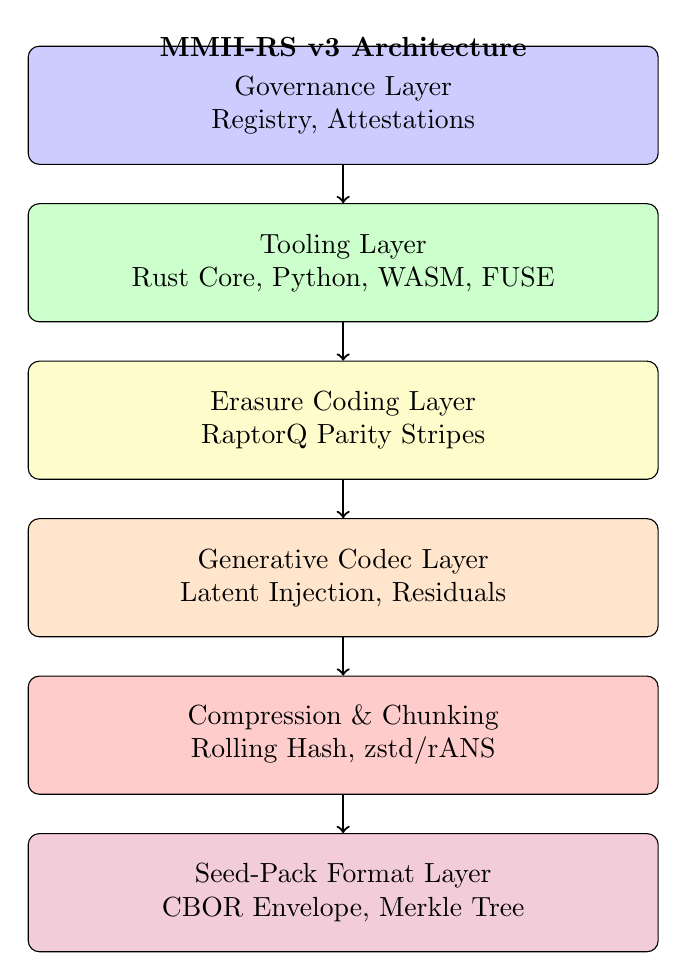
\begin{tikzpicture}[
    box/.style={rectangle, draw, minimum width=2cm, minimum height=1cm, align=center},
    layer/.style={rectangle, draw, rounded corners, minimum width=8cm, minimum height=1.5cm, align=center},
    arrow/.style={->, thick}
]
    % Layers
    \node[layer, fill=blue!20] (governance) at (0,0) {Governance Layer\\Registry, Attestations};
    \node[layer, fill=green!20] (tooling) at (0,-2) {Tooling Layer\\Rust Core, Python, WASM, FUSE};
    \node[layer, fill=yellow!20] (fec) at (0,-4) {Erasure Coding Layer\\RaptorQ Parity Stripes};
    \node[layer, fill=orange!20] (codec) at (0,-6) {Generative Codec Layer\\Latent Injection, Residuals};
    \node[layer, fill=red!20] (chunking) at (0,-8) {Compression \& Chunking\\Rolling Hash, zstd/rANS};
    \node[layer, fill=purple!20] (format) at (0,-10) {Seed-Pack Format Layer\\CBOR Envelope, Merkle Tree};
    
    % Arrows
    \draw[arrow] (governance) -- (tooling);
    \draw[arrow] (tooling) -- (fec);
    \draw[arrow] (fec) -- (codec);
    \draw[arrow] (codec) -- (chunking);
    \draw[arrow] (chunking) -- (format);
    
    % Labels
    \node[above] at (0,0.5) {\textbf{MMH-RS v3 Architecture}};
\end{tikzpicture}
\caption{MMH-RS layered architecture showing the six core components from governance down to the seed-pack format layer.}
\label{fig:architecture}
\end{figure} 